\renewcommand{\arraystretch}{1.5}
\chapter{Exkurse}
\TitleSUB{Ganz viele viele Erklärungen, Beispiele und Extras?}
\elable{chp:EXKURSE}

\section{Wie man sich eine eigene Vorlesung bastelt}
\begin{bemerkung}[Disclaimer]
    Aktuell kann \Jake Daten noch nicht wirklich dynamisch laden. Es ist zwar möglich Quellpfade zu ändern,
    allerdings würde das bedeuten die komplette Ordnerstruktur zu reproduzieren und die notwendingen Standarts selbst zur Verfügung stellen zu müssen. Deswegen wird die Vorlesung direkt in Lilly integriert.
\end{bemerkung}

Der Datenordner, in dem sich die Vorlesung unter \blatex{Lilly/source/Data/Semester/Definitions/:lan:Vorlesung:ran:} befindet, besitzt eine relativ verpflichtende Struktur, die sich geplant mit \LILLYxBOXxVersion{2.1.0} geändert hat. Hier die Übersicht der Ordnerstruktur ab \blatex{Lilly/source/Data/}:\par
\begin{minipage}{0.65\linewidth}Die Verzeichnisse können weitere Ordner enthalten diese werden allerdings (wie die \T{Readme.md}) nicht von Lilly beachtet. Sie können dafür weitere Informationen für Vorlesungen liefern, die dann von diesen Eingebunden werden. Die Definition \T{GENERAL.tex}\footnote{Auch bezüglich der Benennung der Konfigurationen ist eine Änderung für \LILLYxBOXxVersion{2.1.0} geplant.} wird immer geladen und kann so allgemeine Definitionen angeben (so zum Beispiel das Setzen des \blankcmd{LILLYxFlavourText}). Alle anderen Konfigurationen tragen den Namen, der der \LILLYxNOTExLibrary{LILLYxKEYVALxPARSER}-Option \T{Vorlesung} oder der \Jake[-]\jmark[Einstellung]{mrk:jakesettings} \T{lilly-vorlesung} übergeben werden können. Ein \emph{mapping} dieser Bezeichner findet in \LILLYxNOTExLibrary{LILLYxPHILOSOPHER} statt.

\paragraph{Die Vorlesungskonfiguration}
Eine Vorlesungskonfiguration wie \T{EIDI.tex} kann eine Menge an Befehlen definieren, in der Regel werden allerdings die folgenden gesetzt, wobei die mit \T{default} markierten Optionen nicht gegeben werden müssen:
\end{minipage}\begin{minipage}{0.35\linewidth}
    \centering\scalebox{0.75}{\begin{fancydir}
        [Semester
            [Definitions
                [GENERAL.tex, ifile]
                [EIDI.tex, file]
                [FG.tex, file]
                [ANA1.tex, file]
                [\ldots, file]
            ]
            [Graphics
                [source
                    [titleimageEIDI.tex, file]
                    [\ldots, file]
                ]
                [makefile, ifile]
                [titleimageEIDI.pdf, file]
                [titleimageFG.pdf, file]
                [titleimageANA1.pdf, file]
            ]
            [Readme.md]
        ]
    \end{fancydir}}
\end{minipage}
\\
% We set the following commands to be registered here even if they aren't
\foreach \x in {TITLE,PROFESSOR,UEBUNGSLEITER,TUTOR,SUBTITLE,FULLTITLE,UEBUNGSHEADER,VORLESUNG}{\anothercmd*[1.0.0]{\x}}
\begin{center}
    \begin{tabularx}{\linewidth}{^l^p{12em}^>{\ltt\scriptsize}p{12em}^r+}
        \toprule
            \headerrow Befehl         & Erklärung                    & \normalsize Beispiel                    & Notiz \\
        \midrule
            \blankcmd{TITLE}          & Name der Vorlesungsreihe     & Grundlagen der Schäferzucht & \\
            \blankcmd{PROFESSOR}      & Name des Dozenten            & Prof. Dr. Dööst             & \\
            \blankcmd{UEBUNGSLEITER}  & Name des Übungsleiters       & Max Mustermän               & \\
            \blankcmd{TUTOR}          & Name des Tutors              & Herr Subertuter             & \\
            \blankcmd{SUBTITLE}       & Untertitel                   & \blankcmd{PROFESSOR}        & Default\\
            \blankcmd{FULLTITLE}      & Titel für die Titelseite     & \blankcmd{TITLE} \textbackslash\textbackslash\blankcmd{fontsize}\{18pt\}\{16pt\} \blankcmd{selectfont}\{\blankcmd{SUBTITLE}\}             & Default\\
            \blankcmd{UEBUNGSHEADER}  & Kopfzeile eines Übungsblatts & \blankcmd{TITLE}\textbackslash\textbackslash Übungsblatt \blankcmd{LILLY@n} & Default\\
            \blankcmd{VORLESUNG}      & Vorlesungs-Schriftzug        & \{ \blankcmd{bfseries} Roffledoffel \} & Default\\
        \bottomrule
    \end{tabularx}\nskip
\end{center}
Besonders sind die Befehle \blankcmd{UEBUNGSLEITER} und \blankcmd{TUTOR}, da diese erst dann gegeben werden \emph{müssen} wenn sie angefordert werden (genau genommen gilt das für alle Befehle, allerdings werden die anderen in einem Mitschrieb benötigt, um zum Beispiel die Titelseite zu generieren).\newline
Weiter ist es möglich, die beiden folgenden Befehle zu setzen, die eine besondere Bedeutung besitzen:%
\foreach \x in {POLITEINTRO,LILLYxTITLExOffset}{\anothercmd*[1.0.0]{\x}}
\begin{center}
    \begin{tabular}{^l^p{12em}^>{\ltt\scriptsize}p{12em}+}
        \toprule
            \headerrow Befehl         & Erklärung                    & \normalsize Beispiel                    \\
        \midrule
            \blankcmd{POLITEINTRO}    & Einleitung für Zusammenfassungen.     & Offensichtlich erhebt dieses Dokument keinen Anspruch\ldots \\
            \blankcmd{LILLYxTITLExOffset}      & Setzt das horizontale Titelbildoffset bei der Zusammenfassung im Falle einer abweichenden Größe.            & 11.6cm \\
        \bottomrule
    \end{tabular}
\end{center}

Zur Definition weiterer Einschränkungen wie zum Beispiel der Sichtbarkeit von \LILLYxNOTExLibrary{LILLYxBOXES} sollten mit \blankcmd{providedef} getätigt, können allerdings auch anderweitig gesetzt werden, wenn es zum Beispiel anders nicht funktioniert.
Hier ein Beispiel für die Vorlesung \T{ANA1}:
\begin{latex}
%%% Diese Datei enthält alle notwendigen Definitionen

%%%%%%%%%%%%%%%%%%%%% General

%% Setzt den Professor
\def!**!\PROFESSOR{Dr. Supermann}
%% Setzt den Übungsleiter
\def!**!\UEBUNGSLEITER{Someone Günther}
%% Setzt den Tutor
\def!**!\TUTOR{Unbekannt}

%% Setzt den Titel
\def!**!\TITLE{Analysis 1 für Inf. und Ing.}
%% Setzt den Untertitel (Standard)
\def!**!\SUBTITLE{\PROFESSOR}
%% Setzt den Titel für ein Übungsblatt (Standard)
\def!**!\UEBUNGSHEADER{\TITLE!**!\\!**!Übungsblatt \LILLY@n }

%% Setzt den Titel für die Titelseite (Standard)
\def!**!\FULLTITLE{\TITLE!**!\\!**!\fontsize{18pt}{16pt}\selectfont{\SUBTITLE} }

%% Setzt den Namen der Vorlesung als Text, siehe !*\blankcmd{anaI}*!
\def!**!\VORLESUNG{\anaI}

%% Setzt das Intro für eine Zusammenfassung
\DeclareRobustCommand{\POLITEINTRO}{\setcounter{TOPICS}{-1}%
    \TOP[disc]{Disclaimer}{Worte des Autors}
    Offensichtlich erhebt %... Hier gekürzt
    \end{center}
}

%%%%%%%%%%%%%%%%%%%%% Layout Control

%% Setze den Abstand für das Titelbild
\providedef{LILLYxColorxTITLExOffset}{10.3cm}
%% Der Zähler für Definitionen wird mit jeder Sektion zurück gesetzt
\providedef{LILLYxBOXxDefinitionxLock}{section}
%% Der Zähler für jeden Satz wird mit jeder Sektion zurück gesetzt
\providedef{LILLYxBOXxSatzxLock}{section}
%% Bemerkungen sollen ohne Box angezeigt werden
\providedef{LILLYxBOXxBemerkungxBox}{FALSE}
%% Beispiele sollen ohne Box angezeigt werden
\providedef{LILLYxBOXxBeispielxBox}{FALSE}
%% Beweise sollen ohne Box angezeigt werden
\providedef{LILLYxBOXxBeweisxBox}{FALSE}
%% Auf Übungsblättern soll kein Tutorheader angezeigt werden
%% (automatisches !*\blankcmd{TUTORBOX}*!) Dies empfiehlt sich für
%% Übungsblätter mit Onlineabgabe, wenn sie gedruckt werden
%% sollen, dann: TRUE
\providedef{LILLYxUBxSHOWTUTOR}{FALSE}

%%%%%%%%%%%%%%%%%%%%% Title Control

%% Setze das Fakultätssymbol
\def!**!\LILLYxFACULTY{\LILLYxFACULTYxMATHE}
%% Setze die Fakultätsfarbe
\def!**!\LILLYxFACULTYxCOLOR{FacultyMathexColor}

%% Komplett optional, wurde für angenehmere Abstände hier eingefügt
\setlength{\itemsep}{0.40\baselineskip}
\end{latex}

Das ist bezüglich der Konfigurationsdatei eigenlich auch schon alles was gemacht werden muss. Jetzt gilt es allerdings noch das dazugehörige Titelbild zu generieren:

\paragraph{Ein Titelbild erstellen}
An sich gibt es keine klare Regel, nach der ein Titelbild generiert werden muss. Es gibt lediglich die folgenden Anforderungen an die sie sich halten sollen:
\begin{ditemize}
    \item Der Name \emph{muss} \T{titelimage<Vorlesung>.pdf} entsprechen und in \T{Graphics} liegen.
    \item Ein Titelbild sollte völlig unabhängig von Lilly erstellt werden.
    \item Ein Titelbild muss komplett in \LaTeX{} erstellt werden. Externe Grafiken werden nicht gestattet.
    \item Die zugehörige \T{.tex}-Datei \emph{muss} mitgeliefert werden und in \T{Graphics/source} liegen, sie wird automatisch vom \emph{makefile} erfasst.
    \item Es muss ein \emph{Makefile} existieren welches alle Titelbilder eines Ordners auf einmal neu generiert, sofern eine Änderung vorliegt. Dieses wird für Lilly bereits mitgeliefert.
\end{ditemize}

\section{Eine Präsentation erstellen}
\elable{mrk:beamerKIZexample}Zum Erstellen von Präsentationen, kommt zusammen mit Lilly das Beamer-Theme \T{lillyKIZ}, welches eine \T{beamer}-Präsentation mit einem anderen Design versieht und die zu verwendenden Befehle modifiziert. Ersteinmal eine Übersicht, wie das Ganze am Ende aussieht:
\begin{tcbraster}[raster columns=3, blankest,colback=white]
    \tcbincludepdf{Data/Documents/BeamerThemelillyKIZ/presentation.pdf}
\end{tcbraster}
Es läuft unabhängig von der kompletten Lilly-Welt und unterstützt (dank der \T{beamer}-Klasse) auch nicht alle Bibliotheken. Das Aussehen gleicht der Powerpoint-Vorlage der Universität Ulm, die Einbindung erfolgt einfach:
\begin{latex}
\documentclass{beamer}
\usetheme{lillyKIZ}
\end{latex}
Anschließend stehen einige Befehle zur Verfügung:

%
%
%

\presentCommand[2.1.0]{settitle}[\manArg{title}\cmdlist\anothercmd[2.1.0]{setheading}\manArg{heading}\cmdlist\anothercmd[2.1.0]{setsubheading}\secline\manArg{subheading}\cmdlist\anothercmd[2.1.0]{setauthor}\manArg{author}\cmdlist\anothercmd[2.1.0]{setsubtitle}\manArg{subtitle}\cmdlist\secline\anothercmd[2.1.0]{setdate}\manArg{date}\cmdlist\anothercmd[2.1.0]{setresourcepath}\manArg{resourcepath}\cmdlist\secline\anothercmd[2.1.0]{settitleimage}\manArg{titleimage}\cmdlist\anothercmd[2.1.0]{settitlewidth}\manArg{titlewidth}\cmdlist\secline\anothercmd[2.1.0]{setlogoimage}\manArg{logoimage}\cmdlist\anothercmd[2.1.0]{setsignature}\manArg{signature}\cmdlist\secline\anothercmd[2.1.0]{setsignatureDarker}\manArg{signatureDarker}]
Setzt die entsprechenden Felder in der Präsentation.

%
%
%

\presentEnvironment[1.0.7]{bulletpoints}[\optArg{itemize args}]
Setzt eine Liste analog zur Vorlage.

%
%
%

\presentEnvironment[1.0.7]{slide}[\optArg[t]{Orientation}\manArg{Title}]
Sollte anstelle von \blankenv{frame} verwendet werden, kümmert sich um die Nummerierung und das korrekte Setzen des Titels.

\begin{bemerkung}[Code für das obige Beispiel]
    Das \jmark[obige]{mrk:beamerKIZexample} Beispiel wurde durch diesen Code erzeugt:
    \ilatex{Data/Documents/BeamerThemelillyKIZ/presentation.tex}
    Er befindet sich (in den Quelldateien der Dokumentation) im folgenden Ordner:  \blatex{Data/Documents/BeamerThemelillyKIZ}.
\end{bemerkung}

\section{Einen Generator kreieren}
\elable{mrk:gpdgenerators}Auf Basis des Gepard-Moduls \jmark[Generators]{gpd:generators} gilt es in diesem Abschnitt einen dem Mitschrieb-Generator ähnlichen Generator für ein Übungsblatt aufzubauen. Da (vor allem bezüglich der Variablen) dieser Aufbau wechselseitig abläuft wird deswegen an den beiden Dateien (der \T{.gpd}-Datei für die Gepard-Definition und der \T{.template}-Datei für das Template) nebenläufig gearbeitet. Zuerst erzeugen wir eine entsprechende Datei \T{uebungsblatt.gpd}:
\begin{gepard}
BEGIN generator:
    name                   = mein-ub
    template-file          = ./uebungsblatt.template
    target-mode            = 1
    brief                  = Generiert ein Übungsblatt.
END;
\end{gepard}
Die verbundene Template-Datei muss übrigens nicht auf die Endung \T{.template} enden, es sorgt nur für eine gewisse Struktur. Wir setzen den Zielmodus auf $1$, da das erwünschte Dokument kein Expandable mehr enthalten soll (idealerweise) und machen uns nun an das Generieren des zugehörigen Templates in \T{uebungsblatt.template}:
\begin{gepard}
>imp>#./uebungsblatt.tex
% Erstellt am ${GEN-DATE} um ${GEN-TIME}
% von: ${AUTHOR}
:
\begin{aufgabe}{Titel}{Punkte}
    Allgemeine Aufgabenbeschreibung\ldots
    \begin{aufgaben}[!**!2!**!]
        \item Teilaufgabe a)
        \item Teilaufgabe b)
        \item Teilaufgabe c)
        \item Teilaufgabe d)
    \end{aufgaben}
\vSplitter
    \begin{aufgaben}
        \item Lösung a)
        \item Lösung b)
        \item Lösung c)
        \item Lösung d)
    \end{aufgaben}
\end{aufgabe}
\end{gepard}
Führen wir das Projekt nun einmal aus (zum Beispiel durch: \bbash{jake -gepardrule-path: ./uebungsblatt.gpd generate :mein-ub}), erhalten wir bereits ein Übungsblatt. Die hierbei mit \T{\$\{GEN-DATE\}} und \T{\$\{GEN-TIME\}} markierten Expandables sind für den Generator besonders und expandieren zum entsprechenden Generierungs-Datum und -Zeitpunkt.
Wir wollen nun allerdings mehr und erzeugen uns erstmal noch ein entsprechendes Configfile dazu, fügen also die folgenden Zeilen unserem Template an:
\begin{gepard}
>imp>#./uebungsblatt.conf
operation   = file_compile
file        = uebungsblatt.tex
:
lilly-modes = uebungsblatt
lilly-show-boxname = false
:
lilly-boxes = ALTERNATE
lilly-signatur-farbe = bondiBlue
:
lilly-nameprefix = ${AUTHOR}!**!-
lilly-author = ${AUTHOR}
:
lilly-n     = 42
\end{gepard}
Bereits durch das Fixieren von \T{lilly-n} auf $42$ macht deutlich, dass es solangsam einmal Zeit wird Variablen abzufragen die wir vom Nutzer benötigen. Für den Anfang genügen uns die Vorlesung, die Übungsblatt-Nummer und, der Name, wobei wir letzteren optional machen. Der \T{generator}-Box fügen wir damit die folgenden Zeilen hinzu:
{\lstfs{8}
\begin{plaingepard}
Vorlesung = Bitte gib die zugehörige Vorlesung an (ANA1, LAII, ...)
Ub-Nr     = Bitte gib die Nummer des Übungsblattes an
cAuthor   = Bitte gib den Namen der Autoren des Übungsblattes an [optional]
\end{plaingepard}
}
Nun können wir die beiden Dateien entsprechend abändern, sodass sie noch die neuen Einstellungen sinnvoll erweietern. So könnte sich zum Beispiel folgendes Template-File ergeben:
\begin{gepard}
>imp>#./|var|${Vorlesung}|var|-|var|${Ub-Nr}|var|.tex

% Erstellt am ${GEN-DATE} um ${GEN-TIME}
% von: ${AUTHOR}
:
\begin{aufgabe}{Titel}{Punkte}
    Allgemeine Aufgabenbeschreibung\ldots
    \begin{aufgaben}[!**!2!**!]
        \item Teilaufgabe a)
        \item Teilaufgabe b)
        \item Teilaufgabe c)
        \item Teilaufgabe d)
    \end{aufgaben}
\vSplitter
    \begin{aufgaben}
        \item Lösung a)
        \item Lösung b)
        \item Lösung c)
        \item Lösung d)
    \end{aufgaben}
\end{aufgabe}

>imp>#./|var|${Vorlesung}|var|-|var|${Ub-Nr}|var|.conf
operation   = file_compile
file        = ./|var|${Vorlesung}|var|-|var|${Ub-Nr}|var|.tex
:
lilly-modes = uebungsblatt
lilly-show-boxname = false
:
lilly-boxes = ALTERNATE
lilly-signatur-farbe = bondiBlue
:
lilly-nameprefix = |var|${cAuthor:${NAMEPREFIX}}|var|-
lilly-author = |var|${cAuthor:${AUTHOR}}|var|
:
lilly-n     = |var|${Ub-Nr:@[AUTONUM]}|var|
\end{gepard}
Im Folgenden nun ein Beispielhafter Ablauf, wie mit diesem Template (unter der Annahme es liegt samt Template im aktuellen Verzeichnis) unter \LILLYxBOXxVersion{2.1.0} ablaufen kann (es wurden zur besseren Optik in diesem format teils Zeilenumbrüche eingefügt). Das Setzen von \T{answer} auf \T{yes}, unterdrückt hierbei die Fragen, ob die entsprechenden Pfade akzpetiert werden:
{\lstfs{8}
\begin{plainbash}
>imp>the-limerent@elizabeth /tmp/ttextmp
> $ ls
uebungsblatt.gpd  uebungsblatt.template

>imp>the-limerent@elizabeth /tmp/ttextmp
> $ jake -gepardrule-path: ./uebungsblatt.gpd generate :mein-ub -answer: yes
Der Generator benötigt ein paar Informationen, die es nun auszufüllen gilt.
Du kannst keinen Wert angeben um eine optionale Angabe zu verweigern.
[cAuthor] Bitte gib den Namen der Autoren des Übungsblattes an [optional]> 
                Florian-S-Dieter-X
[Vorlesung] Bitte gib die zugehörige Vorlesung an (ANA1, LAII, ...)> FG
[Ub-Nr] Bitte gib die Nummer des Übungsblattes an> 9
Generiere auf Basis von: ./uebungsblatt.template
Der von dir gewählte Generator möchte eine Datei hier hin platzieren: ./FG-9.tex
Der von dir gewählte Generator möchte eine Datei hier hin platzieren: ./FG-9.conf

>imp>the-limerent@elizabeth /tmp/ttextmp
> $ jake FG-9.conf
Kompiliere Dokument: "./FG-9.tex" für: Florian-S-Dieter-X (florian.sihler@web.de)
Information: Aufgrund des Name-Mappings werden deine Einstellungen angepasst. 
Die Regeln im Folgenden werden jeweils angezeigt und angwendet:
    - FG
> Lösche temporäre Dateien...
Lilly PRE-Hook[debug] für PRE evaluiert zu: Verwende die Log-Datei: 
            /tmp/lilly-temp-log**8077425150559038754.temp
Lilly IN0-Hook[compile-0] für IN0 evaluiert zu: Kompiliere 1/2 für: 
            ./FG-9-OUT/Florian-S-Dieter-X-FG-9.pdf
Lilly IN1-Hook[compile-1] für IN1 evaluiert zu: Kompiliere 2/2 für: 
        ./FG-9-OUT/Florian-S-Dieter-X-FG-9.pdf
Generierung von "./FG-9-OUT/Florian-S-Dieter-X-FG-9.pdf" (ALTERNATE) abgeschlossen. 
        (Zeit: 3.295s)
> Lösche temporäre Dateien...
Kompilieren abgeschlossen!
\end{plainbash}
}
Die entstehende datei sieht wie folgt aus (der hier automatisch auftauchende Tutor sollte in einem richtigen Template natürlich überschrieben werden und wurde hier entsprechend zensiert, das Blatt wurde zudem mit der Nummer $14$ generiert, allerdings sollte das für die Demo nichts verändern.)
\begin{center}
    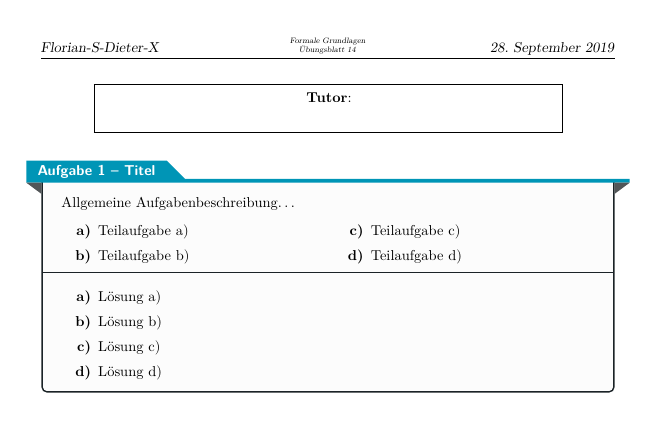
\includegraphics[width=0.9\linewidth]{Data/Bilder/GeneratorUBBeispiel}
\end{center}
Übrigens, der hier gebaute Generator existiert (ungefähr) so bereits in Lilly unter dem Namen \T{uebungsblatt}!
% Todo: fix fancydir